\documentclass[12pt, titlepage]{article}

\usepackage{fullpage}
\usepackage[numbers,square,sort&compress]{natbib}
\usepackage{multirow}
\usepackage{booktabs}
\usepackage{tabularx}
\usepackage{graphicx}
\usepackage{float}
\usepackage{xr}
\usepackage{hyperref}
\hypersetup{
    colorlinks,
    citecolor=blue,
    filecolor=black,
    linkcolor=red,
    urlcolor=blue
}

\input{../../Comments.text}
\input{../../Common.text}
\externaldocument[SRS-]{../../SRS-IEEE/SRS}
\newcommand{\sysname}{The ASSURE Project}

\newcounter{acnum}
\newcommand{\actheacnum}{AC\theacnum}
\newcommand{\acref}[1]{AC\ref{#1}}

\newcounter{ucnum}
\newcommand{\uctheucnum}{UC\theucnum}
\newcommand{\uref}[1]{UC\ref{#1}}

\newcounter{mnum}
\newcommand{\mthemnum}{M\themnum}
\newcommand{\mref}[1]{M\ref{#1}}
\newcommand{\frref}[1]{FR\ref{SRS-#1}}
\newcommand{\nfrref}[1]{NFR\ref{SRS-#1}}
\newcommand{\drref}[1]{DR\ref{SRS-#1}}
\newcommand{\airref}[1]{AIR\ref{SRS-#1}}
\newcommand{\issue}[1]{\href{https://github.com/shivyam/cas-course-optimization/issues/#1}{\##1}}

% IEEEtran.bst control: write repeated author names in full instead of a dash.
% \bstctlcite is defined by the IEEEtran class; article needs it here.
\makeatletter
\def\bstctlcite{\@ifnextchar[{\@bstctlcite}{\@bstctlcite[@auxout]}}
\def\@bstctlcite[#1]#2{\@bsphack\@for\@citeb:=#2\do{%
  \edef\@citeb{\expandafter\@firstofone\@citeb}%
  \if@filesw\immediate\write\csname #1\endcsname{\string\citation{\@citeb}}\fi}%
  \@esphack}
\makeatother

\begin{document}
\bstctlcite{IEEEexample:BSTcontrol}

\title{Module Guide for \progname{}} 
\author{\authname}
\date{\today}

\maketitle

\pagenumbering{roman}

\section{Revision History}

\begin{tabularx}{\textwidth}{p{3cm}p{2cm}X}
\toprule {\bf Date} & {\bf Version} & {\bf Notes}\\
\midrule
Date 1 & 1.0 & Notes\\
Date 2 & 1.1 & Notes\\
\bottomrule
\end{tabularx}

\newpage

\section{Reference Material}

This section records information for easy reference. 

\subsection{Abbreviations and Acronyms}

\renewcommand{\arraystretch}{1.2}
\begin{tabular}{l l} 
  \toprule		
  \textbf{symbol} & \textbf{description}\\
  \midrule 
  AC & Anticipated Change\\
  DAG & Directed Acyclic Graph \\
  M & Module \\
  MG & Module Guide \\
  OS & Operating System \\
  R & Requirement\\
  SC & Scientific Computing \\
  SRS & Software Requirements Specification\\
  \progname & Explanation of program name\\
  UC & Unlikely Change \\
  \wss{etc.} & \wss{...}\\
  \bottomrule
\end{tabular}\\

\newpage

\tableofcontents

\listoftables

\listoffigures

\newpage

\pagenumbering{arabic}

\section{Introduction}

Decomposing a system into modules is a commonly accepted approach to developing
software.  A module is a work assignment for a programmer or programming
team~\citep{ParnasEtAl1984}.  We advocate a decomposition
based on the principle of information hiding~\citep{Parnas1972a}.  This
principle supports design for change, because the ``secrets'' that each module
hides represent likely future changes.  Design for change is valuable in SC,
where modifications are frequent, especially during initial development as the
solution space is explored.  

Our design follows the rules layed out by Parnas et al.~\citep{ParnasEtAl1984}, as follows:
\begin{itemize}
\item System details that are likely to change independently should be the
  secrets of separate modules.
\item Each data structure is implemented in only one module.
\item Any other program that requires information stored in a module's data
  structures must obtain it by calling access programs belonging to that module.
\end{itemize}

After completing the first stage of the design, the Software Requirements
Specification (SRS), the Module Guide (MG) is developed~\citep{ParnasEtAl1984}. The MG
specifies the modular structure of the system and is intended to allow both
designers and maintainers to easily identify the parts of the software.  The
potential readers of this document are as follows:

\begin{itemize}
\item New project members: This document can be a guide for a new project member
  to easily understand the overall structure and quickly find the
  relevant modules they are searching for.
\item Maintainers: The hierarchical structure of the module guide improves the
  maintainers' understanding when they need to make changes to the system. It is
  important for a maintainer to update the relevant sections of the document
  after changes have been made.
\item Designers: Once the module guide has been written, it can be used to
  check for consistency, feasibility, and flexibility. Designers can verify the
  system in various ways, such as consistency among modules, feasibility of the
  decomposition, and flexibility of the design.
\end{itemize}

The rest of the document is organized as follows. Section
\ref{SecChange} lists the anticipated and unlikely changes of the software
requirements. Section \ref{SecMH} summarizes the module decomposition that
was constructed according to the likely changes. Section \ref{SecConnection}
specifies the connections between the software requirements and the
modules. Section \ref{SecMD} gives a detailed description of the
modules. Section \ref{SecTM} includes two traceability matrices. One checks
the completeness of the design against the requirements provided in the SRS. The
other shows the relation between anticipated changes and the modules. Section
\ref{SecUse} describes the use relation between modules.

\section{Anticipated and Unlikely Changes} \label{SecChange}

This section lists possible changes to the system. According to the likeliness
of the change, the possible changes are classified into two
categories. Anticipated changes are listed in Section \ref{SecAchange}, and
unlikely changes are listed in Section \ref{SecUchange}.


\subsection{Anticipated Changes} \label{SecAchange}

Anticipated changes are the source of the information that is to be hidden
inside the modules. Ideally, changing one of the anticipated changes will only
require changing the one module that hides the associated decision. The approach
adapted here is called design for change.

\acref{acLLM} to \acref{acScope} come from the likely changes in the
SRS~\citep{TeamBVSH2026SRS}; the SRS change is named in brackets.
\acref{acDBMS} to \acref{acOverride} are design decisions that the SRS does not
cover.

\begin{description}
\item[\refstepcounter{acnum} \actheacnum \label{acLLM}:] The language model
  used for extraction and where it runs.
\item[\refstepcounter{acnum} \actheacnum \label{acFormat}:] The format of
  submitted course outlines, for example DOCX or \LaTeX{} in addition to PDF.
\item[\refstepcounter{acnum} \actheacnum \label{acPolicy}:] The McMaster and
  CAS course outline policy rules.
\item[\refstepcounter{acnum} \actheacnum \label{acCEAB}:] The CEAB
  accreditation criteria, the graduate attribute list and the master course
  sheet.
\item[\refstepcounter{acnum} \actheacnum \label{acGA}:] How graduate
  attributes are identified from learning outcome text.
\item[\refstepcounter{acnum} \actheacnum \label{acDensity}:] How assessment
  density per cohort and week is computed and shown.
\item[\refstepcounter{acnum} \actheacnum \label{acCohort}:] How courses are
  grouped into student cohorts, including electives and cross-listed courses.
\item[\refstepcounter{acnum} \actheacnum \label{acCalendar}:] Academic calendar
  dates: term dates, recesses, examination periods and ban periods.
\item[\refstepcounter{acnum} \actheacnum \label{acSuggest}:] The method used to
  suggest alternative assessment dates.
\item[\refstepcounter{acnum} \actheacnum \label{acNotify}:] How results reach
  users. Results are currently only shown on the dashboard.
\item[\refstepcounter{acnum} \actheacnum \label{acExport}:] The export file
  format.
\item[\refstepcounter{acnum} \actheacnum \label{acAuth}:] How users log in,
  for example local accounts or McMaster single sign-on.
\item[\refstepcounter{acnum} \actheacnum \label{acSource}:] The source of
  course data, for example enrolment or timetable data from Mosaic.
\item[\refstepcounter{acnum} \actheacnum \label{acScope}:] The set of courses
  covered, for example graduate courses or other departments.
\item[\refstepcounter{acnum} \actheacnum \label{acDBMS}:] The database
  management system and the storage schema.
\item[\refstepcounter{acnum} \actheacnum \label{acPrompt}:] The prompt wording
  and the output structure asked of the model.
\item[\refstepcounter{acnum} \actheacnum \label{acHardware}:] The hardware and
  operating system of the CAS server on which the system runs.
\item[\refstepcounter{acnum} \actheacnum \label{acLayout}:] The layout and
  look of the web pages.
\item[\refstepcounter{acnum} \actheacnum \label{acOverride}:] The rules for
  which findings an administrator may accept, and what is recorded when one is
  accepted.
\end{description}




\subsection{Unlikely Changes} \label{SecUchange}

The module design should be as general as possible. However, a general system is
more complex. Sometimes this complexity is not necessary. Fixing some design
decisions at the system architecture stage can simplify the software design. If
these decision should later need to be changed, then many parts of the design
will potentially need to be modified. Hence, it is not intended that these
decisions will be changed.

\uref{ucAuthority} to \uref{ucFirstYear} come from the unlikely changes in the
SRS~\citep{TeamBVSH2026SRS}. \uref{ucDeterministic} and \uref{ucConfirm} are
design decisions.

\begin{description}
\item[\refstepcounter{ucnum} \uctheucnum \label{ucAuthority}:] Instructors
  keep final authority over assessment dates; the system never changes a date
  on its own.
\item[\refstepcounter{ucnum} \uctheucnum \label{ucOutline}:] Course outlines
  remain the main source of assessment information.
\item[\refstepcounter{ucnum} \uctheucnum \label{ucCode}:] The first digit of a
  course number gives its year level.
\item[\refstepcounter{ucnum} \uctheucnum \label{ucRoles}:] There are two user
  roles: CAS administrator and instructor.
\item[\refstepcounter{ucnum} \uctheucnum \label{ucOffering}:] Every
  assessment belongs to one course offering.
\item[\refstepcounter{ucnum} \uctheucnum \label{ucWeb}:] The system is used
  through a web browser.
\item[\refstepcounter{ucnum} \uctheucnum \label{ucFirstYear}:] First-year
  courses stay out of scope.
\item[\refstepcounter{ucnum} \uctheucnum \label{ucDeterministic}:] Date,
  ban-period and weight checks are done by the system's own code, never by the
  language model.
\item[\refstepcounter{ucnum} \uctheucnum \label{ucConfirm}:] No model output
  is used for the calendar, the workload analysis or the compliance checks
  until a user has confirmed it.
\end{description}


\section{Module Hierarchy} \label{SecMH}

This section provides an overview of the module design. Modules are summarized
in a hierarchy decomposed by secrets in Table \ref{TblMH}. The modules listed
below, which are leaves in the hierarchy tree, are the modules that will
actually be implemented.

\begin{description}
\item [\refstepcounter{mnum} \mthemnum \label{mHH}:] Hardware-Hiding Module
\item [\refstepcounter{mnum} \mthemnum \label{mIntake}:] Outline Intake Module
\item [\refstepcounter{mnum} \mthemnum \label{mExtract}:] Extraction Module
\item [\refstepcounter{mnum} \mthemnum \label{mReview}:] Extraction Review Module
\item [\refstepcounter{mnum} \mthemnum \label{mSchedule}:] Assessment Schedule Module
\item [\refstepcounter{mnum} \mthemnum \label{mWorkload}:] Workload Analysis Module
\item [\refstepcounter{mnum} \mthemnum \label{mPolicy}:] Policy Compliance Module
\item [\refstepcounter{mnum} \mthemnum \label{mGA}:] Graduate Attribute Check Module
\item [\refstepcounter{mnum} \mthemnum \label{mFindings}:] Findings and Override Module
\item [\refstepcounter{mnum} \mthemnum \label{mDashboard}:] Dashboard Module
\item [\refstepcounter{mnum} \mthemnum \label{mSuggest}:] Date Suggestion Module
\item [\refstepcounter{mnum} \mthemnum \label{mExport}:] Export Module
\item [\refstepcounter{mnum} \mthemnum \label{mAccess}:] Access Control Module
\item [\refstepcounter{mnum} \mthemnum \label{mUI}:] Web UI Module
\item [\refstepcounter{mnum} \mthemnum \label{mControl}:] Request Controller Module
\item [\refstepcounter{mnum} \mthemnum \label{mCohort}:] Cohort Module
\item [\refstepcounter{mnum} \mthemnum \label{mCalendar}:] Academic Calendar Module
\item [\refstepcounter{mnum} \mthemnum \label{mReader}:] Document Reader Module
\item [\refstepcounter{mnum} \mthemnum \label{mLLM}:] LLM Client Module
\item [\refstepcounter{mnum} \mthemnum \label{mStore}:] Data Store Module
\end{description}

\begin{table}[h!]
\centering
\begin{tabular}{p{0.3\textwidth} p{0.6\textwidth}}
\toprule
\textbf{Level 1} & \textbf{Level 2}\\
\midrule

{Hardware-Hiding Module} & Hardware-Hiding (\mref{mHH})\\
\midrule

\multirow{16}{0.3\textwidth}{Behaviour-Hiding Module}
& Outline Intake (\mref{mIntake})\\
& Extraction (\mref{mExtract})\\
& Extraction Review (\mref{mReview})\\
& Assessment Schedule (\mref{mSchedule})\\
& Workload Analysis (\mref{mWorkload})\\
& Policy Compliance (\mref{mPolicy})\\
& Graduate Attribute Check (\mref{mGA})\\
& Findings and Override (\mref{mFindings})\\
& Dashboard (\mref{mDashboard})\\
& Date Suggestion (\mref{mSuggest})\\
& Export (\mref{mExport})\\
& Access Control (\mref{mAccess})\\
& Web UI (\mref{mUI})\\
& Request Controller (\mref{mControl})\\
& Cohort (\mref{mCohort})\\
& Academic Calendar (\mref{mCalendar})\\
\midrule

\multirow{3}{0.3\textwidth}{Software Decision Module}
& Document Reader (\mref{mReader})\\
& LLM Client (\mref{mLLM})\\
& Data Store (\mref{mStore})\\
\bottomrule

\end{tabular}
\caption{Module Hierarchy}
\label{TblMH}
\end{table}


\section{Connection Between Requirements and Design} \label{SecConnection}

The design of the system is intended to satisfy the requirements developed in
the SRS. In this stage, the system is decomposed into modules. The connection
between requirements and modules is listed in Table~\ref{TblRT}.

%\wss{The intention of this section is to document decisions that are made
%  ``between'' the requirements and the design.  To satisfy some requirements,
%  design decisions need to be made.  Rather than make these decisions implicit,
%  they are explicitly recorded here.  For instance, if a program has security
%  requirements, a specific design decision may be made to satisfy those
%  requirements with a password.}

\begin{itemize}
\item Only the LLM client (\mref{mLLM}) knows which model is used and how it is called. The current model
  is Gemma 4 E2B, a preliminary choice that may change. The model runs on CAS
  servers, so no outline text leaves CAS infrastructure, and no student
  personal information is sent to the model (\drref{DR_Hosting},
  \airref{AIR_Input_Privacy}). The models Gemma 4 E2B (\issue{38}), Llama 3.2 3B (\issue{40}),
  and Qwen3 4B (\issue{39}) can be swapped in without changing any other module.
\item The Extraction module (\mref{mExtract}) gives the model the outline text only as data and checks
  every reply against the expected structure before it is stored
  (\airref{AIR_Output_Validation}). Each extracted value keeps the passage and
  page it came from (\airref{AIR_Output_Source}), which the Document Reader
  (\mref{mReader}) provides.
\item The Extraction Review module (\mref{mReview}) holds the review state of every extracted
  value. The workload, policy and graduate attribute checks ask it whether a
  course is confirmed before they run (\frref{FR_Extract_Review},
  \airref{AIR_Output_Review}, \uref{ucConfirm}).
\item The Workload Analysis (\mref{mWorkload}) and Policy Compliance (\mref{mPolicy}) modules
  compute ban-period conflicts, weight totals and TBD dates without the model
  (\uref{ucDeterministic}).
\item The Workload Analysis module gives the number of assessments per cohort and 
week; it does not compare it with a department threshold.
\item The Graduate Attribute Check (\mref{mGA}) compares the attributes in a confirmed 
outline with the master course sheet in code (\airref{AIR_Input_Text},
  \drref{DR_Confidentiality}).
\item The Request Controller (\mref{mControl}) asks Access Control (\mref{mAccess}) for the
  current user and role before calling any other module (\frref{FR_Access_Login}, 
  \frref{FR_Access_Roles}, \frref{FR_Access_Timeout}, \drref{DR_Access}, \nfrref{NFR_Security}).
\item The Findings and Override module (\mref{mFindings}) records each accepted 
finding with the administrator, the reason and the time. The Dashboard module
  (\mref{mDashboard}) reports what is missing or wrong for each course and
  whether the term is fully planned.
\item Only the Data Store (\mref{mStore}) talks to the database, and it keeps 
outlines, extracted data and findings for the retention period (\drref{DR_Retention}).
\end{itemize}


\section{Module Decomposition} \label{SecMD}

Modules are decomposed according to the principle of ``information hiding''
proposed by Parnas et al.~\citep{ParnasEtAl1984}. The \emph{Secrets} field in a module
decomposition is a brief statement of the design decision hidden by the
module. The \emph{Services} field specifies \emph{what} the module will do
without documenting \emph{how} to do it. For each module, a suggestion for the
implementing software is given under the \emph{Implemented By} title. If the
entry is \emph{OS}, this means that the module is provided by the operating
system or by standard programming language libraries.  \emph{\progname{}} means the
module will be implemented by the \progname{} software.

Only the leaf modules in the hierarchy have to be implemented. If a dash
(\emph{--}) is shown, this means that the module is not a leaf and will not have
to be implemented.

\subsection{Hardware Hiding Modules (\mref{mHH})}

\begin{description}
\item[Secrets:]The data structure and algorithm used to implement the virtual
  hardware.
\item[Services:]Serves as a virtual hardware used by the rest of the
  system. This module provides the interface between the hardware and the
  software. So, the system can use it to display outputs or to accept inputs.
\item[Implemented By:] OS
\end{description}

\subsection{Behaviour-Hiding Module}

\begin{description}
\item[Secrets:] The contents of the required behaviours.
\item[Services:] Includes programs that provide externally visible behaviour of
  the system as specified in the SRS~\citep{TeamBVSH2026SRS}. This module serves
  as a communication layer between the hardware-hiding module and the software
  decision module. The programs in this module will need to change if there are
  changes in the SRS.
\item[Implemented By:] --
\end{description}

\subsubsection{Outline Intake Module (\mref{mIntake})}

\begin{description}
\item[Secrets:] How submitted files are checked, named and kept.
\item[Services:] Accepts one or many course outlines in one upload, rejects
  files that are not supported or too large, keeps the original file and starts
  extraction for each accepted outline.
\item[Implemented By:] \sysname
\item[Type of Module:] Library
\end{description}

\subsubsection{Extraction Module (\mref{mExtract})}

\begin{description}
\item[Secrets:] The prompts, the output structure and the parsing and
  validation rules used to turn outline text into course data, including how
  graduate attributes are identified when an outline does not list them.
\item[Services:] Produces, for one outline, its assessments (name, type, date
  and weight) and its learning outcomes with their graduate attributes. Each
  value carries its source passage and page. Missing values and dates marked TBD
  are reported as missing, never guessed.
\item[Implemented By:] \sysname
\item[Type of Module:] Library
\end{description}

\subsubsection{Extraction Review Module (\mref{mReview})}

\begin{description}
\item[Secrets:] The review state of each extracted value.
\item[Services:] Shows extracted data so a user can correct and confirm it,
  and tells other modules whether a course's data has been confirmed.
\item[Implemented By:] \sysname
\item[Type of Module:] Abstract Object
\end{description}

\subsubsection{Assessment Schedule Module (\mref{mSchedule})}

\begin{description}
\item[Secrets:] How tentative and confirmed dates are kept for each assessment.
\item[Services:] Lets an instructor enter and change tentative dates for their
  own courses, records approved date changes, and asks for the affected
  analysis to be re-run after every change. It never changes a date without the
  instructor's approval.
\item[Implemented By:] \sysname
\item[Type of Module:] Abstract Object
\end{description}

\subsubsection{Workload Analysis Module (\mref{mWorkload})}

\begin{description}
\item[Secrets:] How assessment density per cohort and week is computed.
\item[Services:] Gives the number of assessments due in each week of term for each cohort, and
lists assessments that fall in restricted periods such as the ban period or the examination period.
\item[Implemented By:] \sysname
\item[Type of Module:] Library
\end{description}

\subsubsection{Policy Compliance Module (\mref{mPolicy})}

\begin{description}
\item[Secrets:] The McMaster and CAS course outline policy rules
\item[Services:] Checks a confirmed outline against the policy: required sections, weights totalling
100\% (including bonus marks), single-weight limits, ban-period rules and dates marked
TBD. Records each problem as a finding.
\item[Implemented By:] \sysname
\item[Type of Module:] Library
\end{description}

\subsubsection{Graduate Attribute Check Module (\mref{mGA})}

\begin{description}
\item[Secrets:] The CEAB graduate attribute list and how it is compared with the master course
sheet.
\item[Services:] Flags graduate attributes in a confirmed outline that are missing from, or do not
match, the master course sheet, and says when a course has no row in the sheet.
\item[Implemented By:] \sysname
\item[Type of Module:] Library
\end{description}

\subsubsection{Findings and Override Module (\mref{mFindings})}

\begin{description}
\item[Secrets:] How findings, accepted findings and their reasons are recorded and audited.
\item[Services:] Lists the findings for each course. Lets an administrator accept a finding with a
reason, which is kept in the audit trail.
\item[Implemented By:] \sysname
\item[Type of Module:] Abstract Object
\end{description}

\subsubsection{Dashboard Module (\mref{mDashboard})}

\begin{description}
\item[Secrets:] How the status of a course and of a term is summarized.
\item[Services:] Presents, for each course the user may see, what is missing, which findings are open
and which values are unconfirmed. Shows whether the term is fully planned before it starts.
\item[Implemented By:] \sysname
\item[Type of Module:] Library
\end{description}

\subsubsection{Date Suggestion Module (\mref{mSuggest})}

\begin{description}
\item[Secrets:] The method used to choose alternative dates.
\item[Services:] Only when an instructor asks, suggests alternative dates for an assessment that
is in a conflict or marked TBD, each with an explanation, and records the instructor’s
decision. Never suggests a date in a restricted period.
\item[Implemented By:] \sysname
\item[Type of Module:] Abstract Object
\end{description}

\subsubsection{Input Format Module (\mref{mInput})}

\begin{description}
\item[Secrets:]The format and structure of the input data.
\item[Services:]Converts the input data into the data structure used by the
  input parameters module.
\item[Implemented By:] [Your Program Name Here]
\item[Type of Module:] [Record, Library, Abstract Object, or Abstract Data Type]
  [Information to include for leaf modules in the decomposition by secrets tree.]
\end{description}


\subsubsection{Cohort Module (\mref{mCohort})}

\begin{description}
\item[Secrets:] The department's master course list and how a course code
  maps to a student cohort.
\item[Services:] Says whether a course code is one of the department's
  courses, gives the cohort (program and year level) a course belongs to, and
  lists the department courses in a cohort. The year level is the first digit
  of the course number.
\item[Implemented By:] \sysname
\item[Type of Module:] Library
\end{description}

\subsubsection{Academic Calendar Module (\mref{mCalendar})}

\begin{description}
\item[Secrets:] The dates of each term: its start and end, its class days, its
  holidays and recesses, and its examination period.
\item[Services:] Gives the dates and class days of a term, the week of term a
  date falls in, and whether a date falls in a holiday, a recess or the
  examination period. The ban period is worked out by Policy Compliance
  (\mref{mPolicy}) from the class days.
\item[Implemented By:] \sysname
\item[Type of Module:] Library
\end{description}

\subsection{Software Decision Module}

\begin{description}
\item[Secrets:] The design decision based on mathematical theorems, physical
  facts, or programming considerations. The secrets of this module are
  \emph{not} described in the SRS.
\item[Services:] Includes data structure and algorithms used in the system that
  do not provide direct interaction with the user. 
  % Changes in these modules are more likely to be motivated by a desire to
  % improve performance than by externally imposed changes.
\item[Implemented By:] --
\end{description}

\subsubsection{Document Reader Module (\mref{mReader})}

\begin{description}
\item[Secrets:] The library and method used to read the text of a document
  and to mark passages in it.
\item[Services:] Returns the text of a course outline page by page, so that
  each extracted value can name the page it came from. Produces a copy of the
  outline with given source passages highlighted, so a reviewer can find each
  value in the original document.
\item[Implemented By:] \sysname, using PyMuPDF~\citep{PyMuPDF}
\item[Type of Module:] Library
\end{description}

\subsubsection{LLM Client Module (\mref{mLLM})}

\begin{description}
\item[Secrets:] Which language model is used, where it runs and how it is
  called.
\item[Services:] Sends instructions and outline text to the language model as
  separate inputs and returns the model's reply. Reports when the model is
  unavailable or does not reply in time. The model runs on CAS servers, so no
  outline text leaves CAS.
\item[Implemented By:] \sysname, using Ollama~\citep{Ollama} to run Gemma 4 E2B (tested in spike
  \href{https://github.com/shivyam/cas-course-optimization/issues/38}{\#38}). This
  model choice is preliminary and may change.
\item[Type of Module:] Library
\end{description}

\subsubsection{Data Store Module (\mref{mStore})}

\begin{description}
\item[Secrets:] The database management system, the storage schema, and how
  the original outline files are kept.
\item[Services:] Saves, loads and queries every stored entity, including the
  original outline files, and keeps records for the retention period.
\item[Implemented By:] \sysname, on MongoDB~\citep{MongoDB}
\item[Type of Module:] Abstract Object
\end{description}


\section{Traceability Matrix} \label{SecTM}

This section shows two traceability matrices: between the modules and the
requirements in the SRS~\citep{TeamBVSH2026SRS} (Tables~\ref{TblRT}
and~\ref{TblRT2}), and between the modules and the anticipated changes
(Table~\ref{TblACT}). The admin override, course status dashboard and term
completeness features are not yet requirements in the SRS, so they are traced
by working name.

\begin{table}[H]
\centering
\begin{tabular}{p{0.38\textwidth} p{0.52\textwidth}}
\toprule
\textbf{Functional Req.} & \textbf{Modules}\\
\midrule
\frref{FR_Intake_Data} & \mref{mIntake}, \mref{mReader}, \mref{mStore}\\
\frref{FR_Extract_Assessment} & \mref{mExtract}, \mref{mLLM}\\
\frref{FR_Extract_LO} & \mref{mExtract}, \mref{mLLM}\\
\frref{FR_Extract_Flag} & \mref{mExtract}\\
\frref{FR_Extract_Review} & \mref{mReview}\\
\frref{FR_Dates_Tentative} & \mref{mSchedule}\\
\frref{FR_Calendar} & \mref{mWorkload}, \mref{mUI}, \mref{mCohort}\\
\frref{FR_Work_Cluster} & \mref{mWorkload}, \mref{mCohort}, \mref{mCalendar}\\
\frref{FR_Work_Policy} & \mref{mWorkload}, \mref{mCalendar}\\
\frref{FR_Reanalyze} & \mref{mSchedule}, \mref{mWorkload}\\
\frref{FR_Suggest_Generation} & \mref{mSuggest}, \mref{mCalendar}\\
\frref{FR_Suggest_NoAuto} & \mref{mSchedule}, \mref{mSuggest}\\
\frref{FR_Comp_Policy} & \mref{mPolicy}, \mref{mCalendar}\\
\frref{FR_Comp_Grad} & \mref{mGA}\\
\frref{FR_Access_Login} & \mref{mAccess}, \mref{mControl}\\
\frref{FR_Access_Roles} & \mref{mAccess}, \mref{mControl}\\
\frref{FR_Access_Timeout} & \mref{mAccess}\\
\frref{FR_Export_CSV} & \mref{mExport}\\
Admin override (working name) & \mref{mFindings}\\
Course status dashboard (working name) & \mref{mDashboard}\\
Term completeness (working name) & \mref{mDashboard}, \mref{mCalendar}\\
\bottomrule
\end{tabular}
\caption{Trace Between Functional Requirements and Modules}
\label{TblRT}
\end{table}

\begin{table}[H]
\centering
\begin{tabular}{p{0.38\textwidth} p{0.52\textwidth}}
\toprule
\textbf{Req.} & \textbf{Modules}\\
\midrule
\drref{DR_Confidentiality} & \mref{mAccess}, \mref{mStore}\\
\drref{DR_Hosting} & \mref{mLLM}\\
\drref{DR_Access} & \mref{mAccess}, \mref{mControl}\\
\drref{DR_Retention} & \mref{mStore}\\
\airref{AIR_Input_Text} & \mref{mExtract}, \mref{mReader}\\
\airref{AIR_Input_Privacy} & \mref{mLLM}\\
\airref{AIR_Output_Struct} & \mref{mExtract}\\
\airref{AIR_Output_Source} & \mref{mExtract}, \mref{mReader}\\
\airref{AIR_Output_Missing} & \mref{mExtract}\\
\airref{AIR_Output_Review} & \mref{mReview}\\
\airref{AIR_Output_Validation} & \mref{mExtract}, \mref{mLLM}\\
\nfrref{NFR_Accuracy} & \mref{mExtract}, \mref{mLLM}, \mref{mPolicy}, \mref{mGA}\\
\nfrref{NFR_Usability} & \mref{mUI}\\
\nfrref{NFR_Maintainability} & All modules (decomposition by secrets)\\
\nfrref{NFR_Portability} & \mref{mHH}, \mref{mUI}\\
\nfrref{NFR_Installability} & \mref{mHH}, \mref{mLLM}, \mref{mStore}\\
\nfrref{NFR_Performance} & \mref{mExtract}, \mref{mLLM}, \mref{mStore}\\
\nfrref{NFR_Reliability} & \mref{mIntake}, \mref{mExtract}, \mref{mLLM}\\
\nfrref{NFR_Security} & \mref{mAccess}, \mref{mControl}\\
\nfrref{NFR_Accessibility} & \mref{mUI}\\
\bottomrule
\end{tabular}
\caption{Trace Between Data, AI and Nonfunctional Requirements and Modules}
\label{TblRT2}
\end{table}

\begin{table}[H]
\centering
\begin{tabular}{p{0.38\textwidth} p{0.52\textwidth}}
\toprule
\textbf{AC} & \textbf{Modules}\\
\midrule
\acref{acLLM} & \mref{mLLM}\\
\acref{acFormat} & \mref{mReader}\\
\acref{acPolicy} & \mref{mPolicy}\\
\acref{acCEAB} & \mref{mGA}\\
\acref{acGA} & \mref{mExtract}\\
\acref{acDensity} & \mref{mWorkload}\\
\acref{acCohort} & \mref{mCohort}\\
\acref{acCalendar} & \mref{mCalendar}\\
\acref{acSuggest} & \mref{mSuggest}\\
\acref{acNotify} & \mref{mDashboard}\\
\acref{acExport} & \mref{mExport}\\
\acref{acAuth} & \mref{mAccess}\\
\acref{acSource} & \mref{mIntake}\\
\acref{acScope} & \mref{mCohort}\\
\acref{acDBMS} & \mref{mStore}\\
\acref{acPrompt} & \mref{mExtract}\\
\acref{acHardware} & \mref{mHH}\\
\acref{acLayout} & \mref{mUI}\\
\acref{acOverride} & \mref{mFindings}\\
\bottomrule
\end{tabular}
\caption{Trace Between Anticipated Changes and Modules}
\label{TblACT}
\end{table}

\section{Use Hierarchy Between Modules} \label{SecUse}

In this section, the uses hierarchy between modules is
provided. Parnas~\citep{Parnas1978} said of two programs A and B that A {\em uses} B if
correct execution of B may be necessary for A to complete the task described in
its specification. That is, A {\em uses} B if there exist situations in which
the correct functioning of A depends upon the availability of a correct
implementation of B.  Figure \ref{FigUH} illustrates the use relation between
the modules. It can be seen that the graph is a directed acyclic graph
(DAG). Each level of the hierarchy offers a testable and usable subset of the
system, and modules in the higher level of the hierarchy are essentially simpler
because they use modules from the lower levels.

\wss{The uses relation is not a data flow diagram.  In the code there will often
be an import statement in module A when it directly uses module B.  Module B
provides the services that module A needs.  The code for module A needs to be
able to see these services (hence the import statement).  Since the uses
relation is transitive, there is a use relation without an import, but the
arrows in the diagram typically correspond to the presence of import statement.}

\wss{If module A uses module B, the arrow is directed from A to B.}

\begin{figure}[H]
\centering
%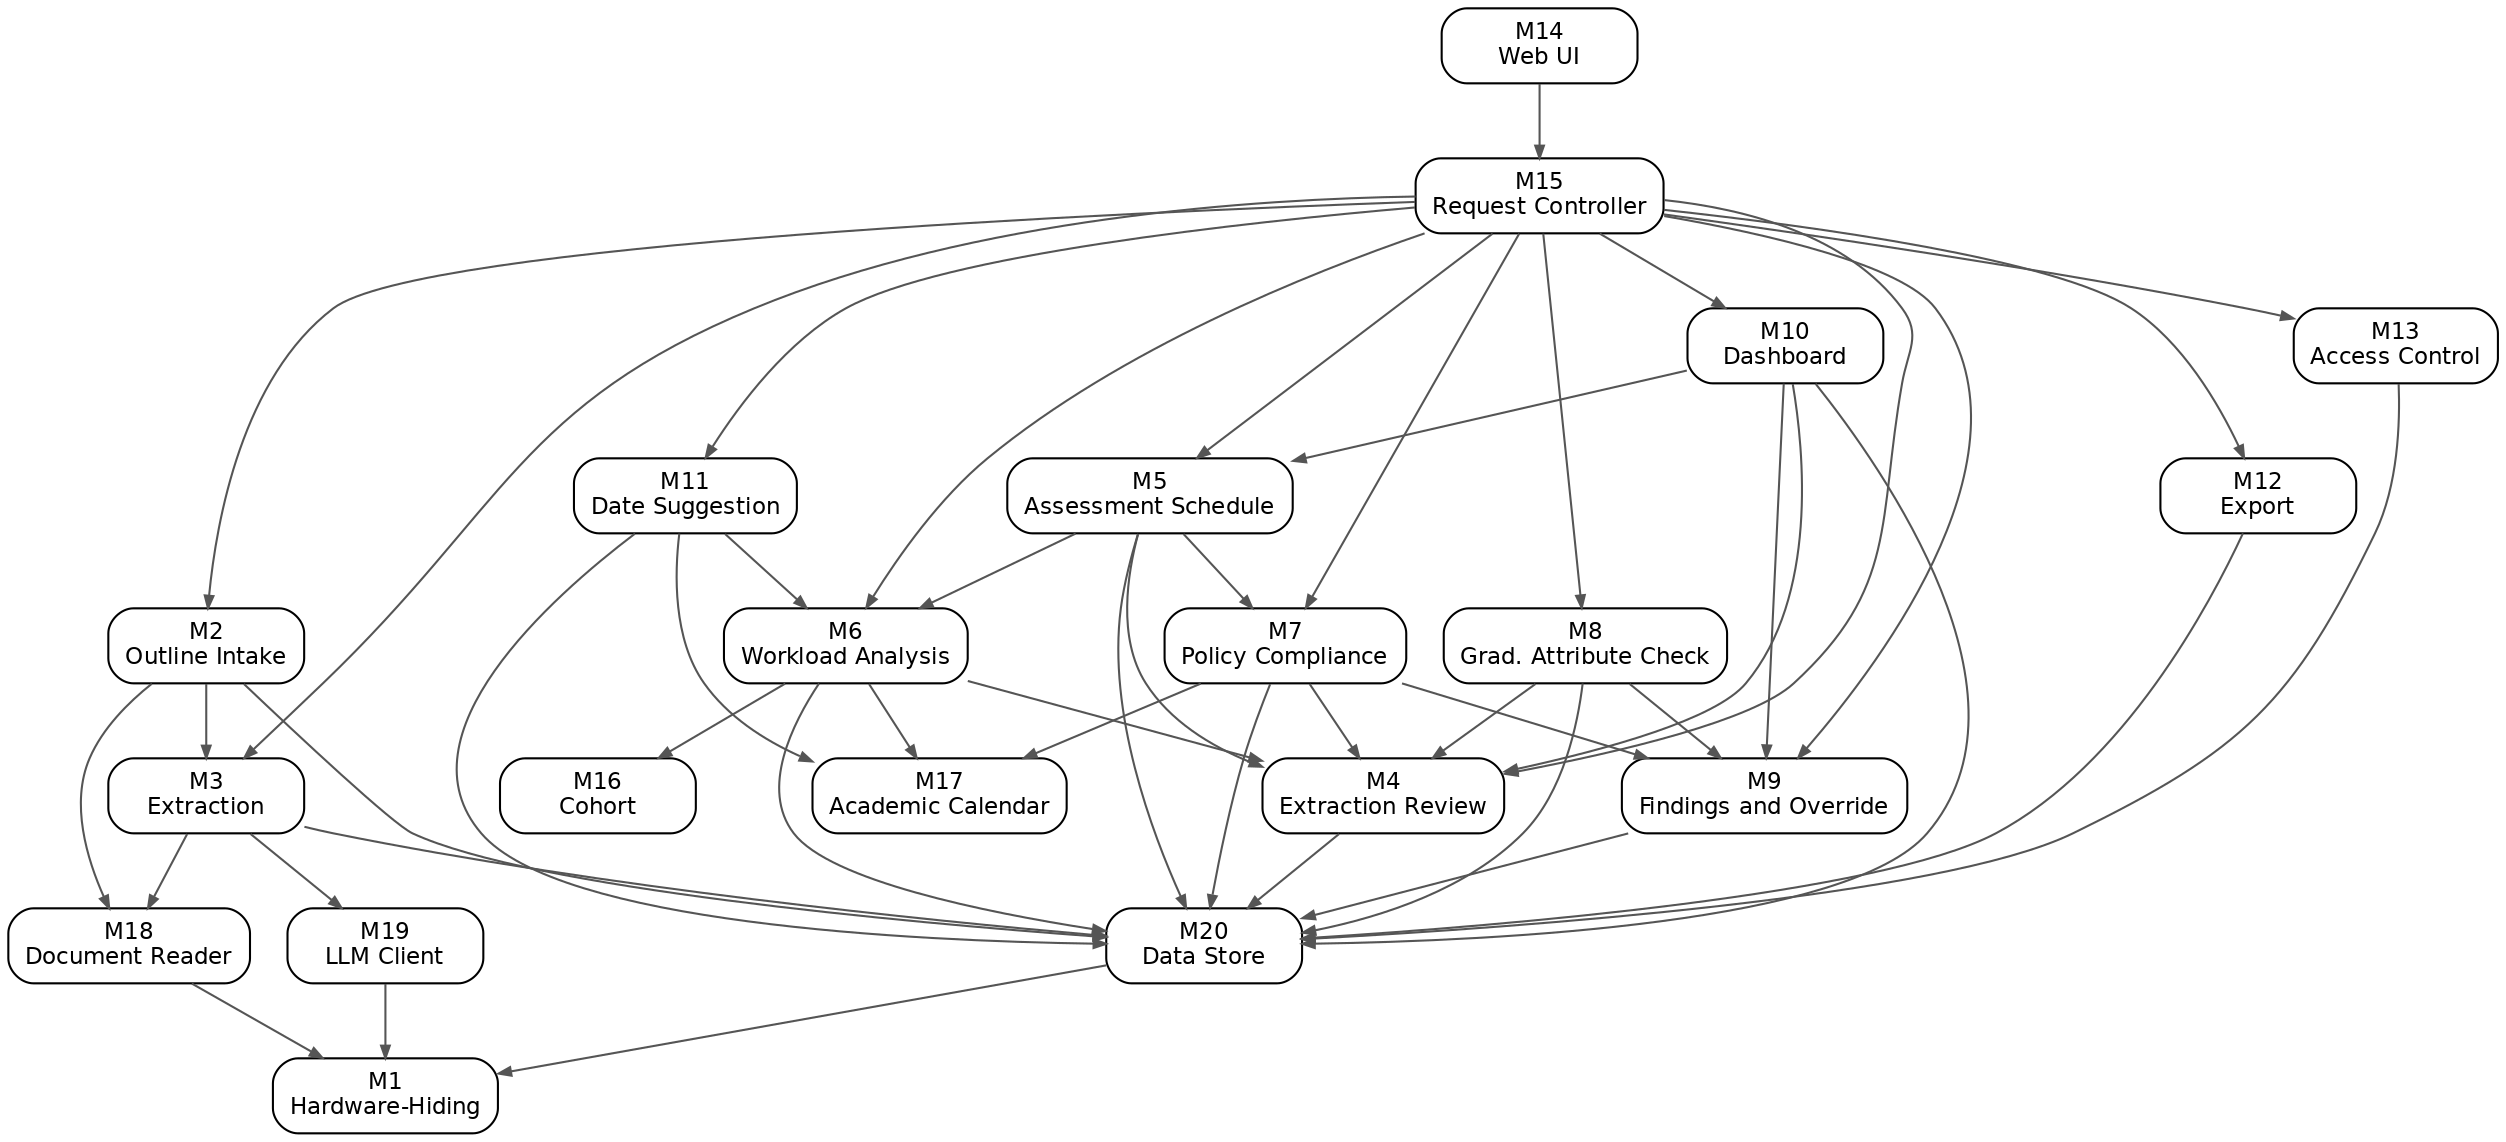
\includegraphics[width=0.7\textwidth]{UsesHierarchy.png}
\caption{Use hierarchy among modules}
\label{FigUH}
\end{figure}

%\section*{References}

\section{User Interfaces}

The system is used through a web browser (\uref{ucWeb}). Pages follow the
McMaster University colour scheme. Table~\ref{TblPages} lists the pages and their purpose. 

\begin{table}[H]
\centering
\begin{tabular}{p{0.22\textwidth} p{0.5\textwidth} p{0.18\textwidth}}
\toprule
\textbf{Page} & \textbf{Purpose} \\
\midrule
Login & Sign in; the session ends after a period without activity\\
Home & Pick a task and see the dashboard summary\\
Upload & Submit one or many outline PDFs\\
Outline preview and review & Check each extracted value against its source
passage, correct it and confirm the outline\\
Calendar & Confirmed and tentative dates, filtered by course, year and program;
assessments per cohort and week\\
Findings & Policy and graduate attribute findings; accept a finding with a
reason\\
Dashboard & Status of each course and whether the term is fully planned \\
Export & Download confirmed assessment data\\
\bottomrule
\end{tabular}
\caption{Web pages}
\label{TblPages}
\end{table}

All planned wireframes are included in Appendix~\ref{app:wireframes}.


\section{Design of Communication Protocols}

%\wss{If there is communication between hardware and software, it may be necessary 
%to explain the design of the communication protocol.  This section should be filled 
%in with NA if it is not appropriate for a given project.}

As there is no hardware component in the system, there is no communication between 
custom hardware and software. Two software interfaces cross a process boundary:

\begin{itemize}
  \item Web UI to Backend: The browser sends HTTP requests to a REST API served under 
  the path \texttt{/api} by the Request Controller (\mref{mControl}), built on 
  FastAPI. Responses are structured data that the Web UI (\mref{mUI}) displays.
  \item Backend to LLM: The LLM Client (\mref{mLLM}) sends
  prompts over HTTP to a model service running on the same CAS server. No 
  request leaves CAS infrastructure.
\end{itemize}


\section{Database Design}

\wss{If a database is a significant component of the project, the database
design should be summarized here.  This section should be filled in with NA if
it is not appropriate for a given project.}

\section{Timeline}

\wss{Schedule of tasks and who is responsible}

\wss{You can point to GitHub if this information is included there}

\section{Generative AI Use Disclosure}

\wss{ChatGPT (version 5) was used to brainstorm ideas for the template for this disclose section.}

\subsection{AI Tools Used}

\wss{Give the name of the AI tool(s) used and the version.}

\subsection{How and Where Used}

\wss{Explain what the tool(s) were used for.  Examples include: brainstorming,
explaining a technical concept, reviewing the document, generating or modifying
text, generating or modifying diagrams, identifying errors or omissions or
inconsistencies.}

\wss{For each of the uses, identify which parts of the document were affected.}

\wss{You do not need to report every interaction, but you should disclose the 
uses that materially contributed to your work}

\subsection{Verification of AI-Generated Content}

\wss{\begin{itemize}
    \item Describe how the team checked AI-generated or AI-assisted material
    before including it in the document.
    \item In particular, verify factual claims, technical assertions,
    requirements, calculations, references, and other information for which an
    AI system may produce incorrect or fabricated results.
    \item \textbf{The team is responsible for the accuracy, completeness,
consistency, and appropriateness of the submitted document, regardless of
whether material was generated by a human or an AI system.}
\end{itemize}}

\appendix

\refstepcounter{section}
\section*{Appendix \thesection: Wireframes} \label{app:wireframes}
\addcontentsline{toc}{section}{Appendix \thesection: Wireframes}

\begin{figure}[H]
    \centering
    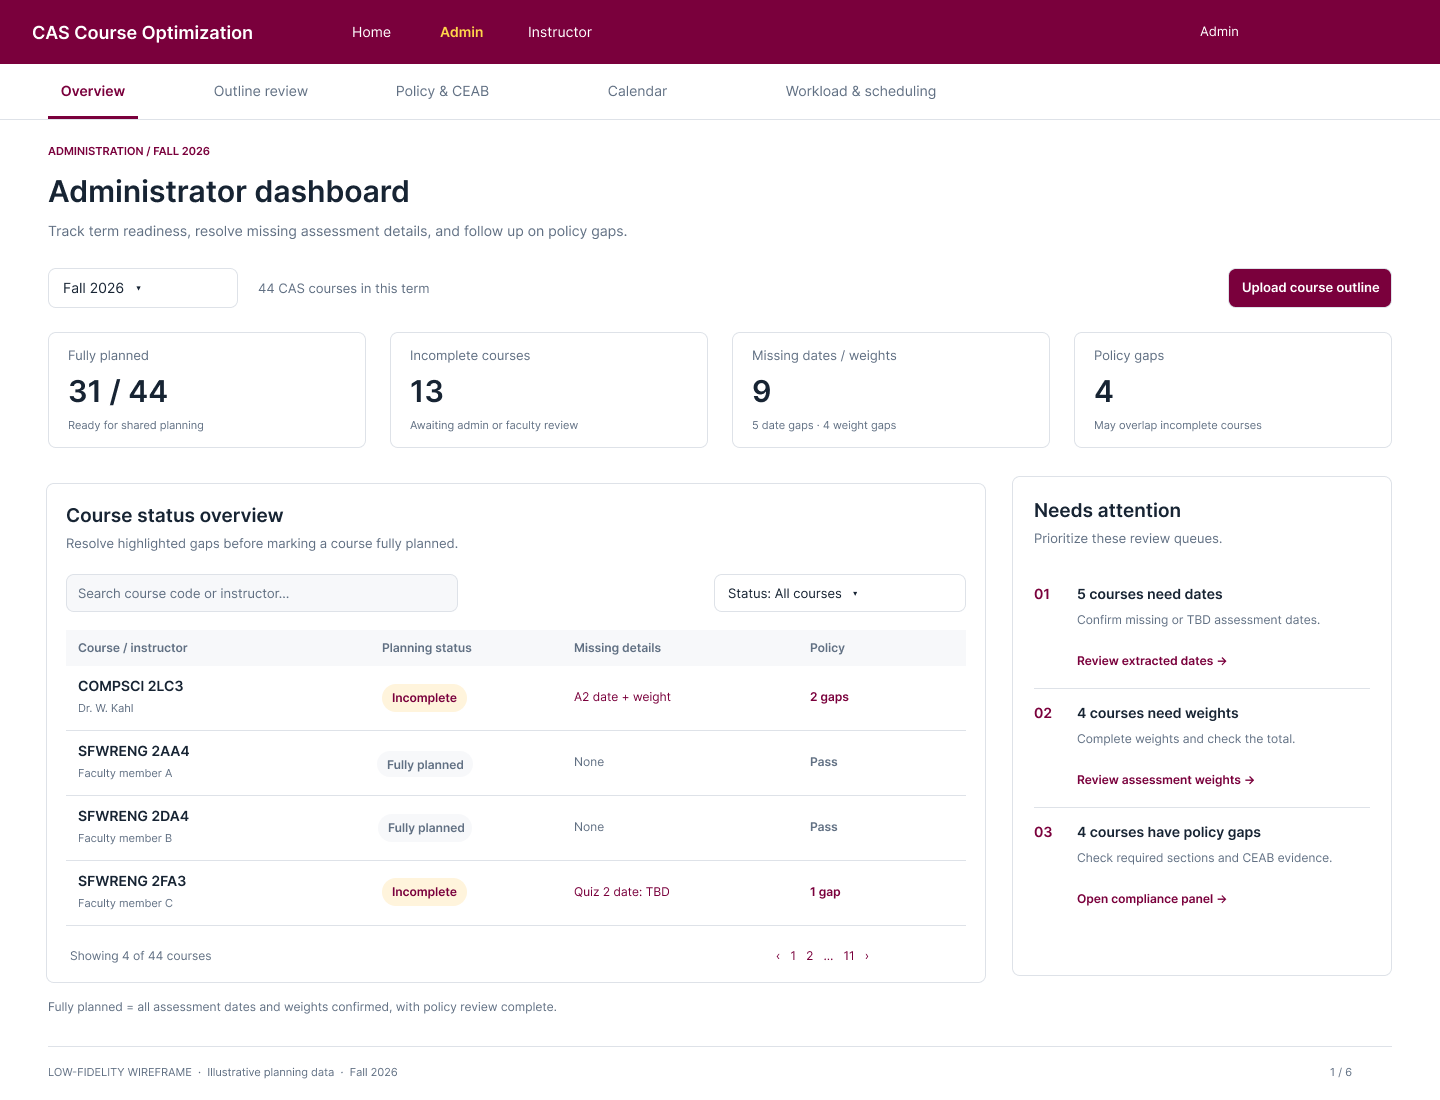
\includegraphics[width=\textwidth]{
        ../../CDs/Wireframe/01. Homepage (Administrator Dashboard).png
    }
    \caption{Administrator dashboard wireframe}
    \label{fig:admin-dashboard}
\end{figure}

\begin{figure}[H]
    \centering
    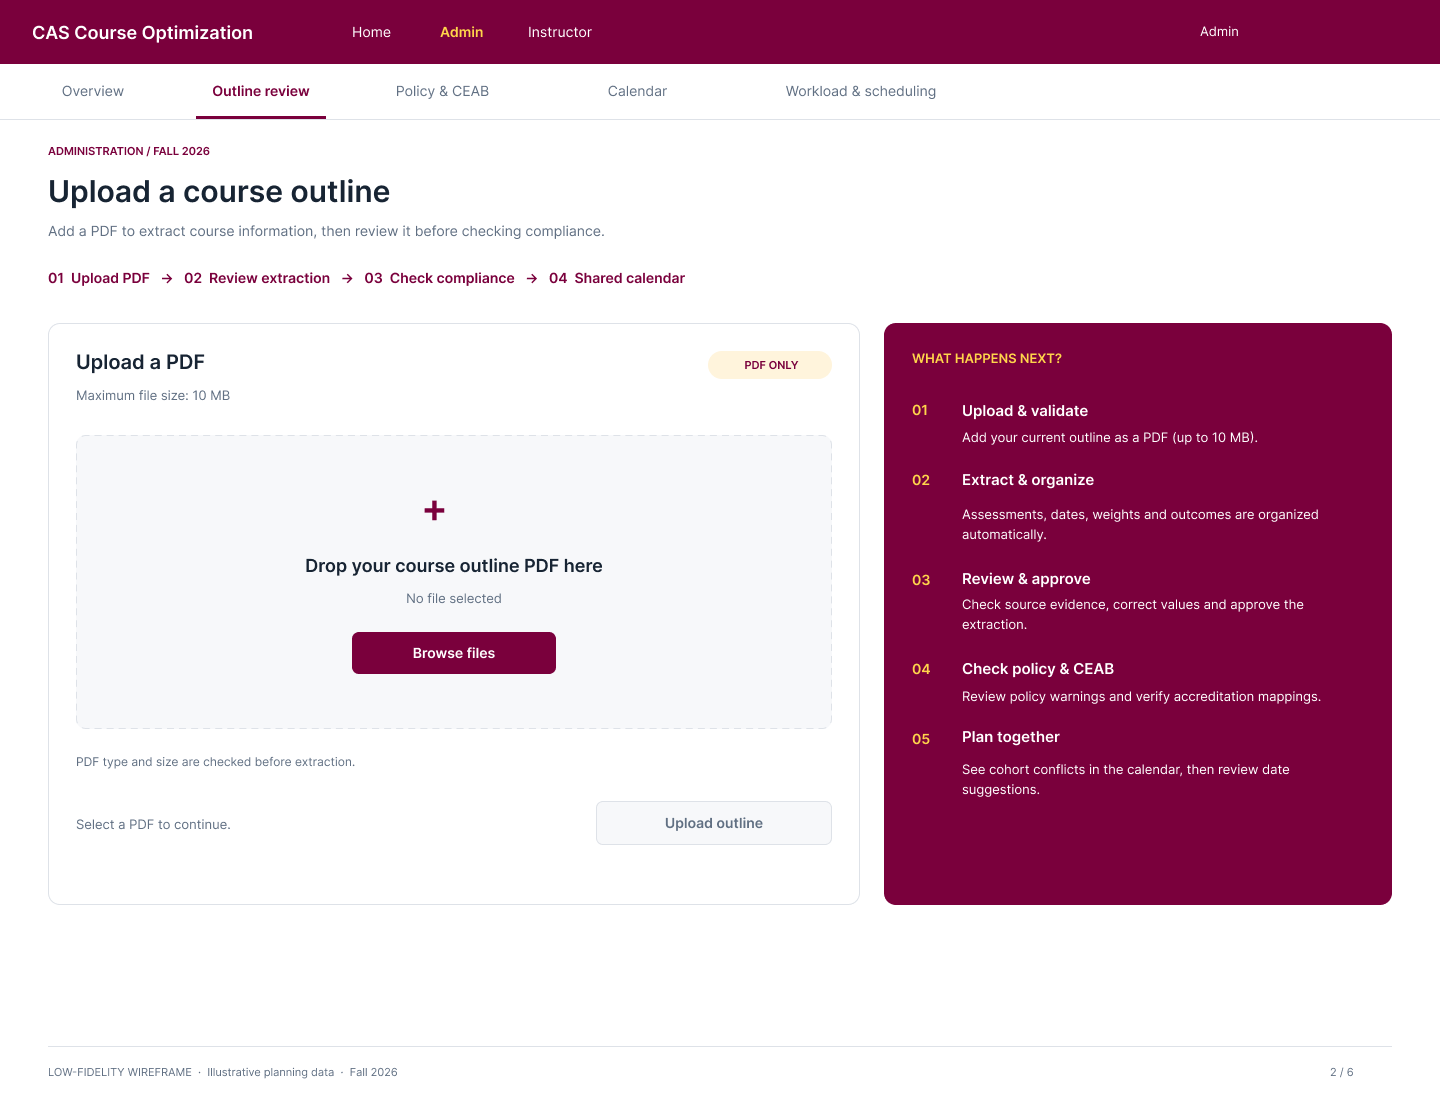
\includegraphics[width=\textwidth]{
        ../../CDs/Wireframe/02a. Course Outline Upload.png
    }
    \caption{Course outline upload wireframe}
    \label{fig:course-outline-upload}
\end{figure}

\begin{figure}[H]
    \centering
    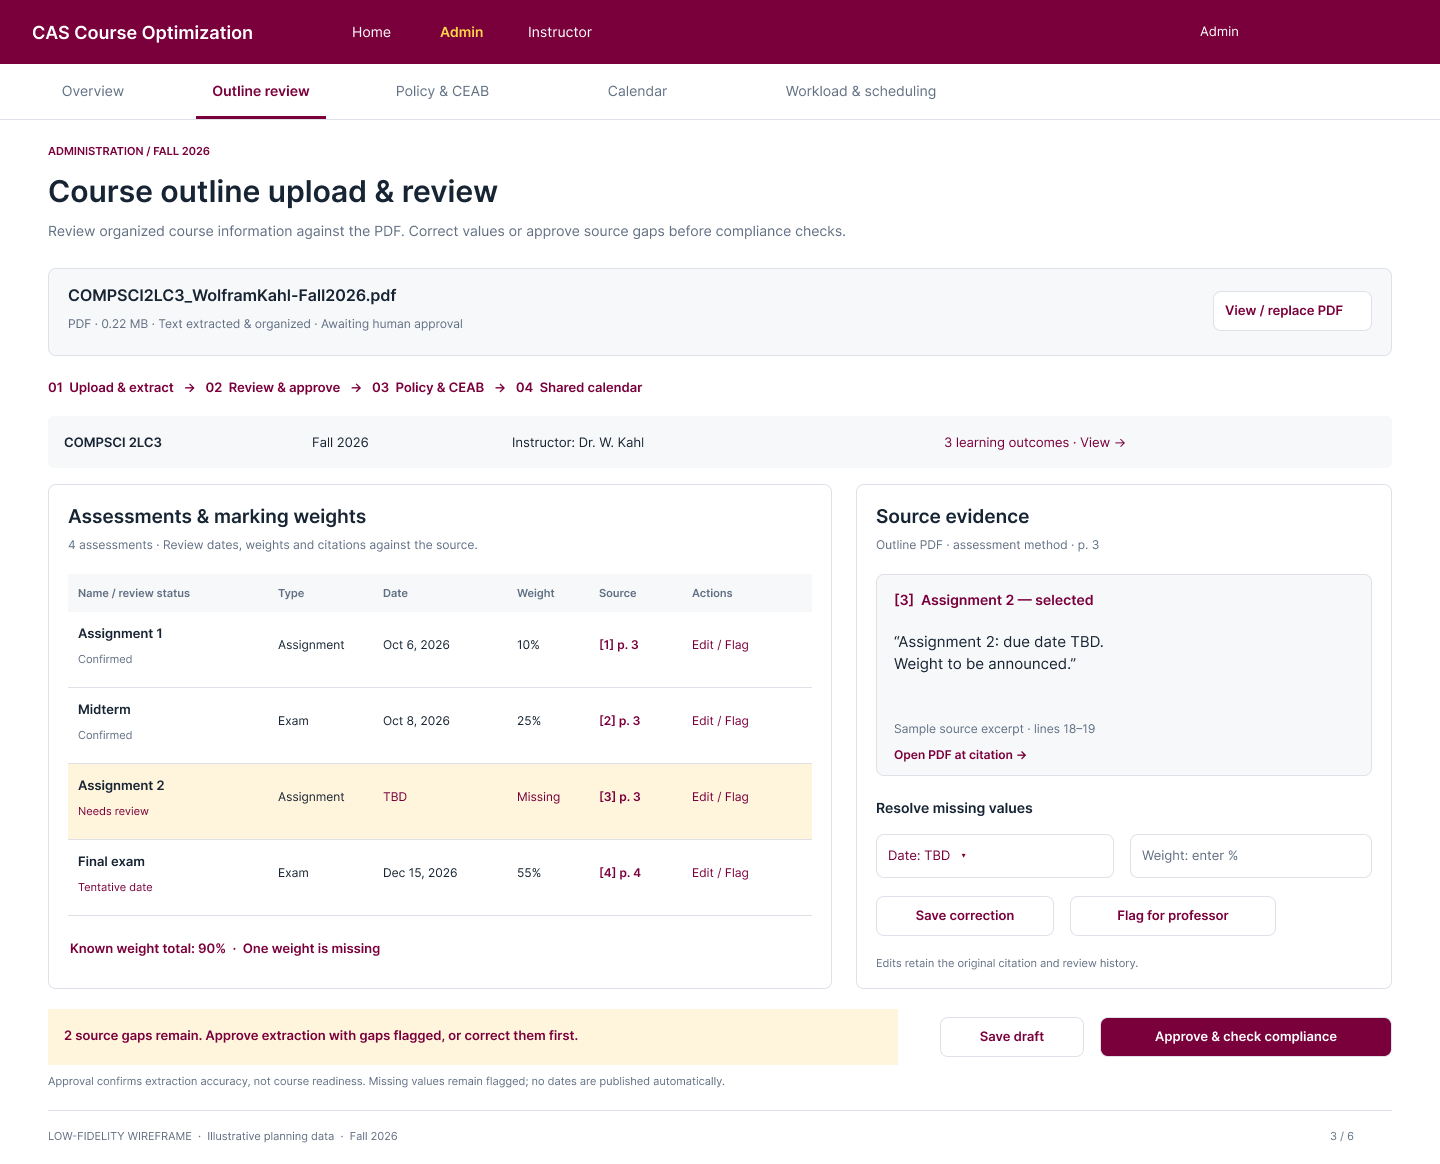
\includegraphics[width=\textwidth]{
        ../../CDs/Wireframe/02b. Course Outline Extraction & Review.png
    }
    \caption{Course outline extraction and review wireframe}
    \label{fig:course-outline-extraction-review}
\end{figure}

\begin{figure}[H]
    \centering
    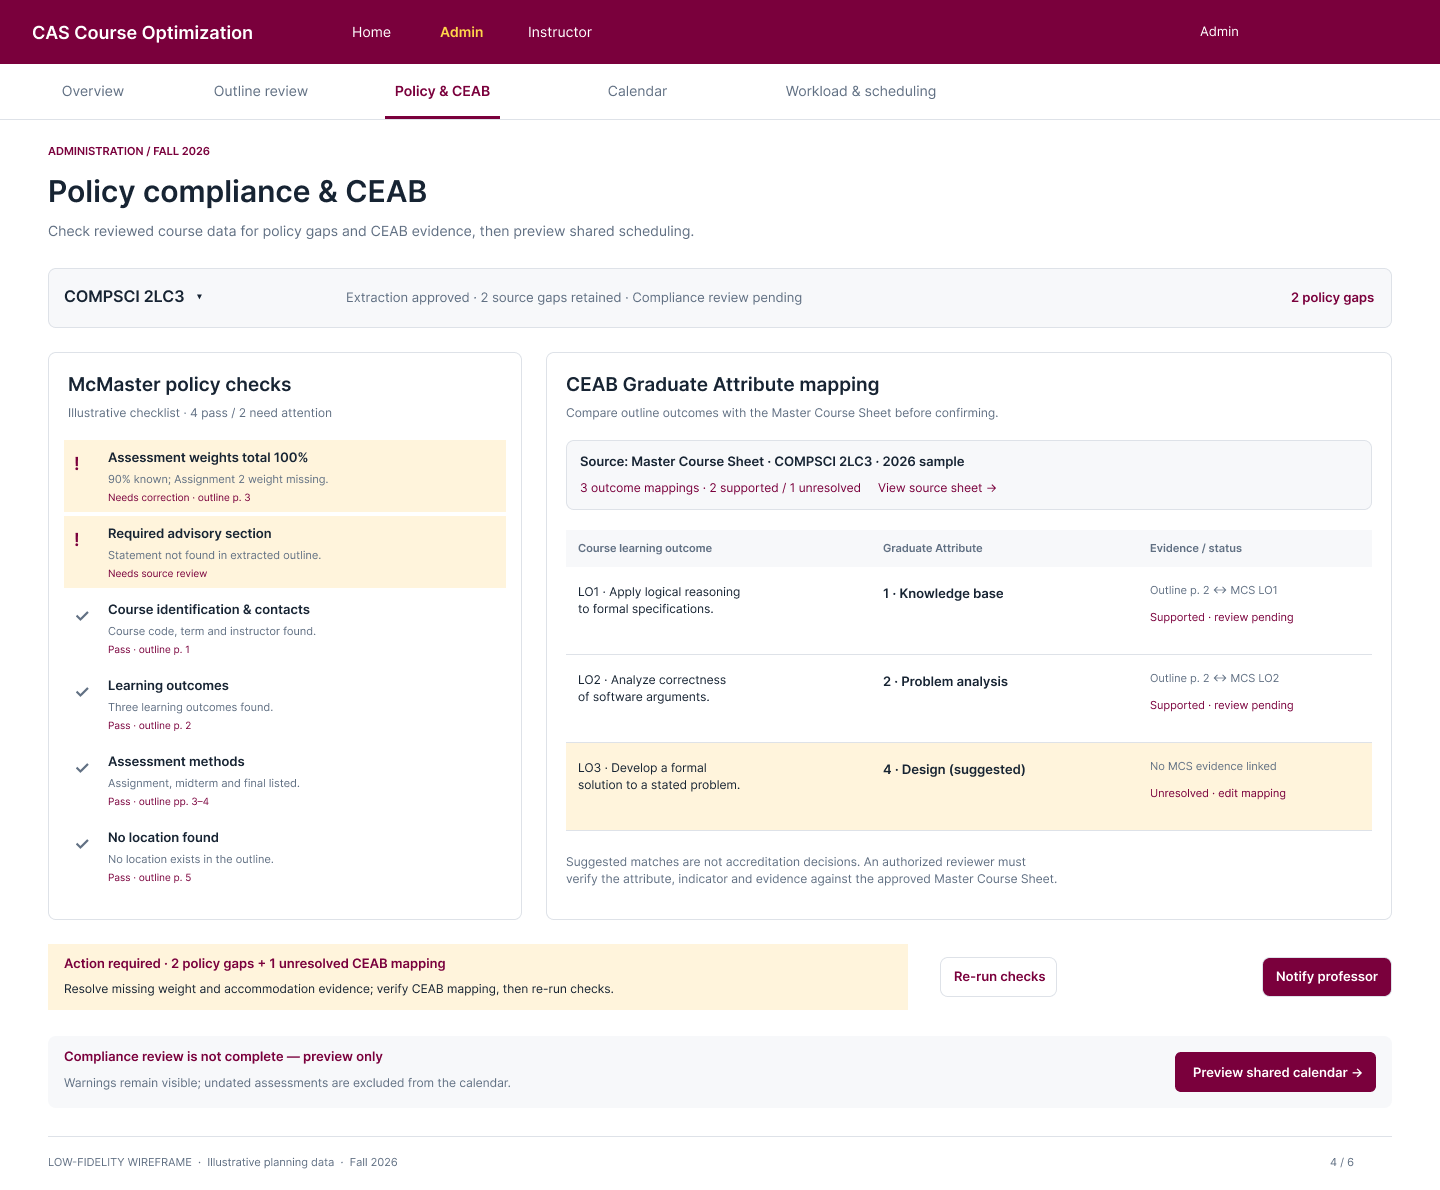
\includegraphics[width=\textwidth]{
        ../../CDs/Wireframe/03. Policy Compliance & CEAB Accreditation.png
    }
    \caption{Policy compliance and CEAB accreditation wireframe}
    \label{fig:policy-compliance-ceab}
\end{figure}


\begin{figure}[H]
    \centering
    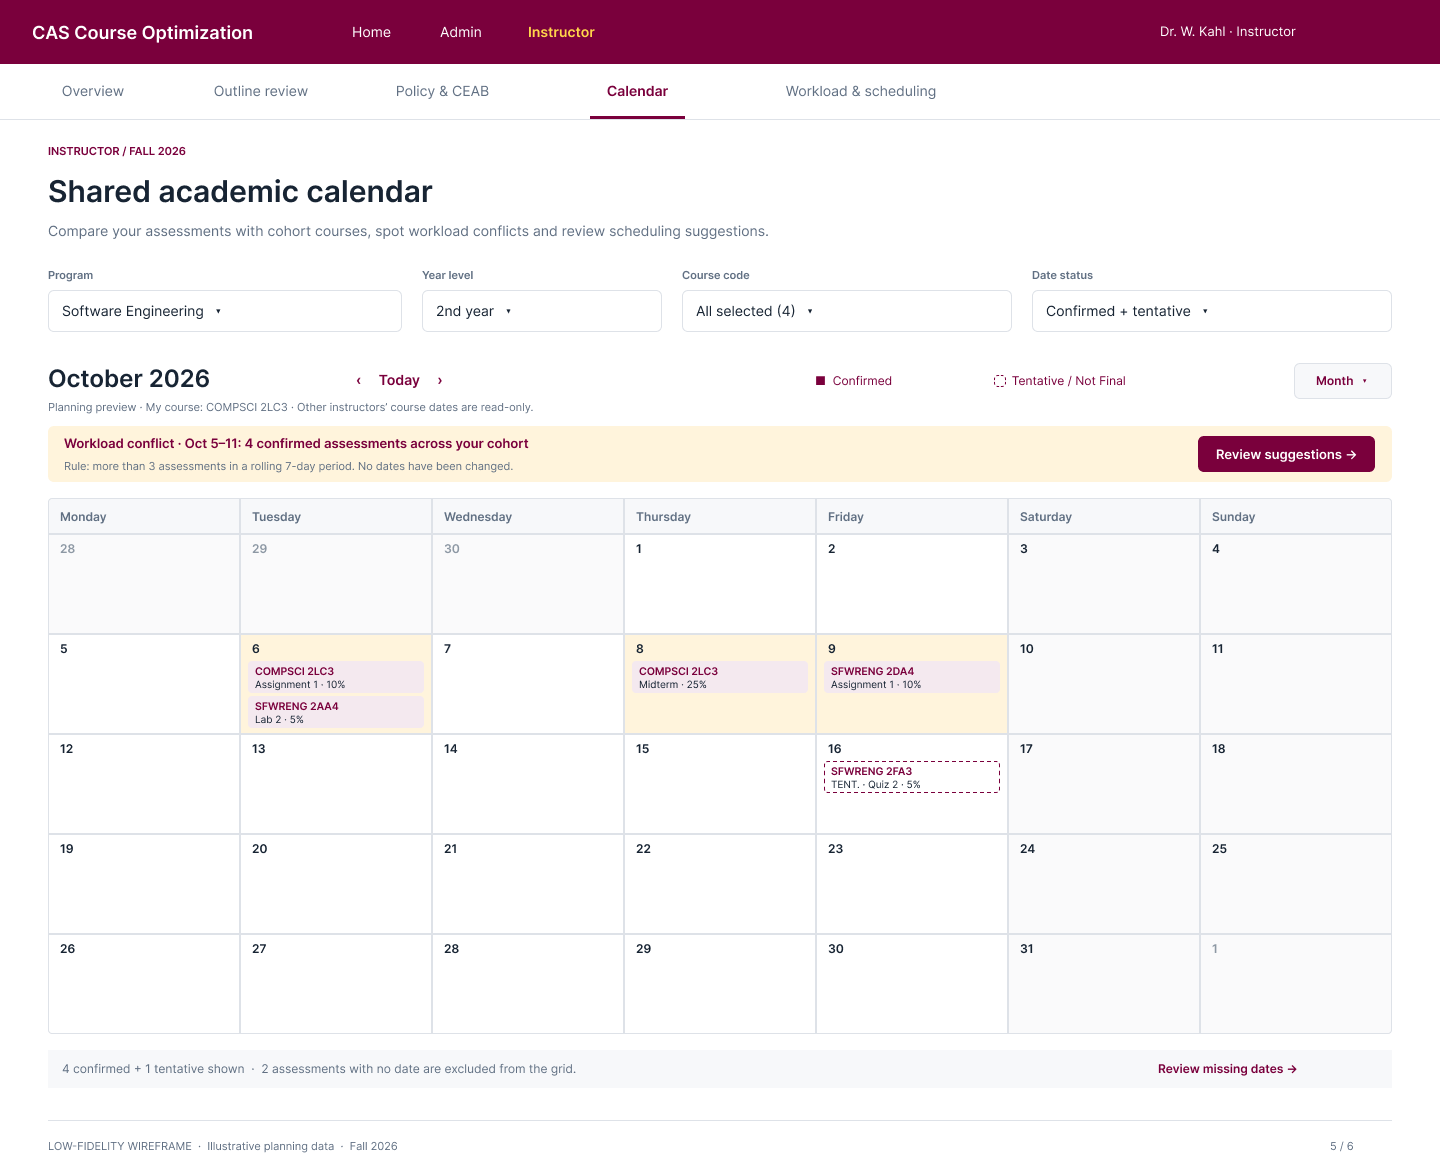
\includegraphics[width=\textwidth]{
        ../../CDs/Wireframe/04. Shared Academic Calendar.png
    }
    \caption{Shared academic calendar wireframe}
    \label{fig:shared-academic-calendar}
\end{figure}

\begin{figure}[H]
    \centering
    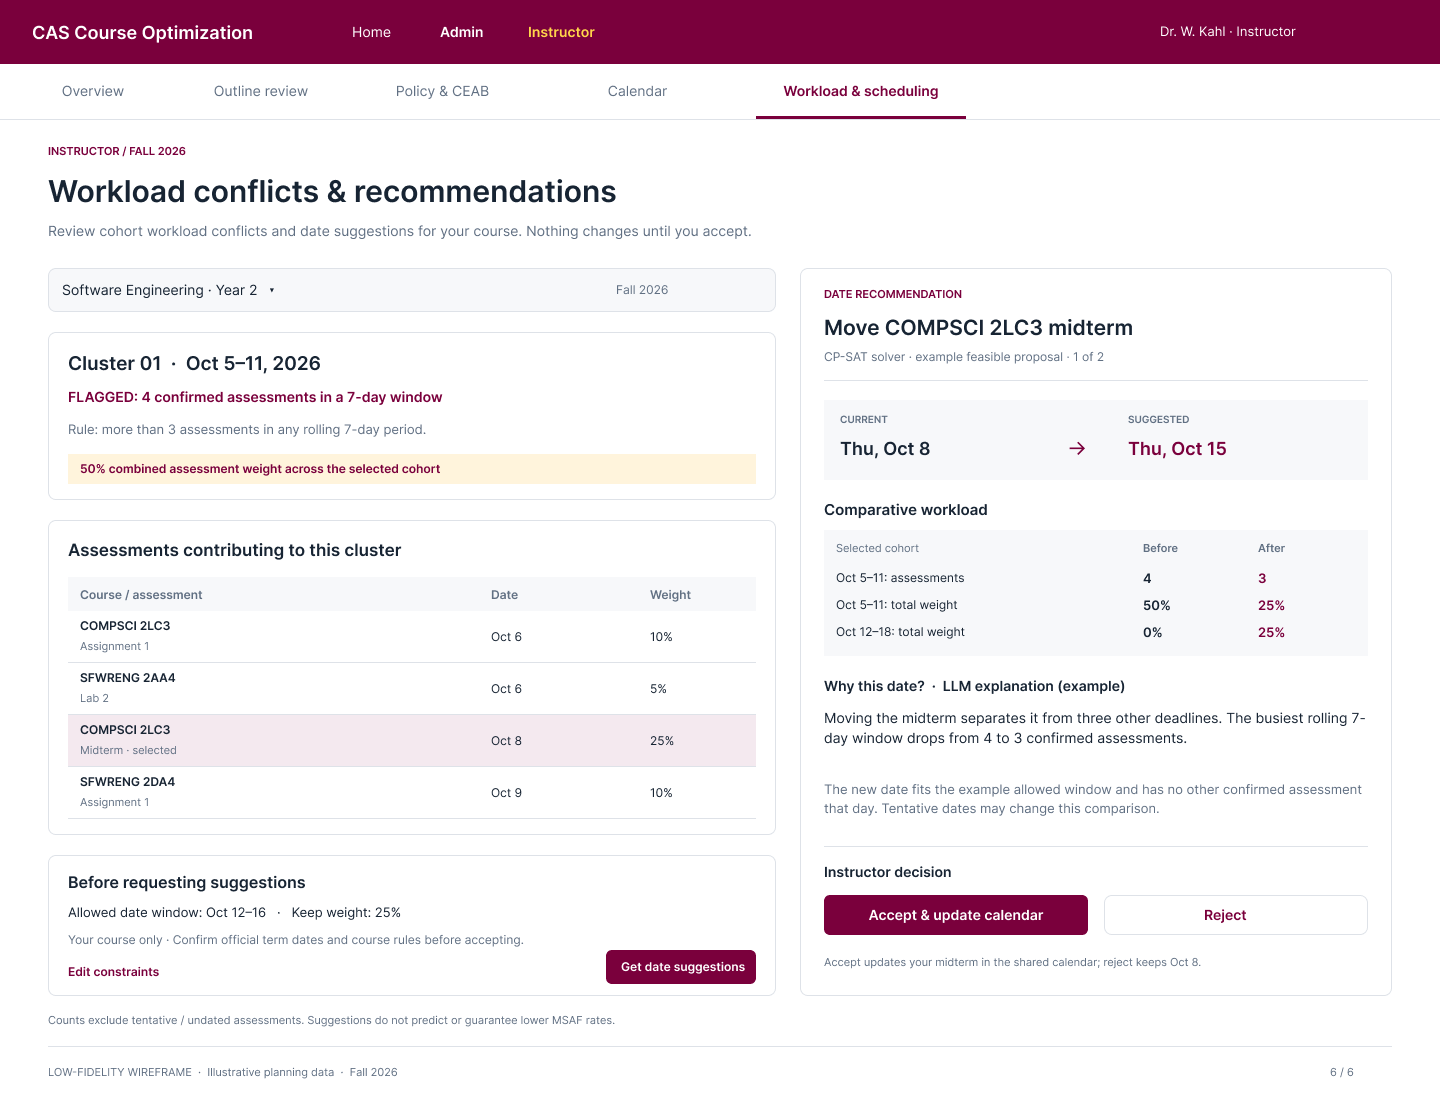
\includegraphics[width=\textwidth]{
        ../../CDs/Wireframe/05. Scheduling Recommendations.png
    }
    \caption{Scheduling recommendations wireframe}
    \label{fig:scheduling-recommendations}
\end{figure}
\newpage{}

% Same IEEE style file as the SRS (IEEEtran.bst is not installed in CI).
\bibliographystyle {../../SRS-IEEE/IEEEtran}
\bibliography{../../../refs/References}

\end{document}